We will follow the same pattern we used in the previous section, so we will start with the robustness for different number of particles for $ \lambda = 5 $.

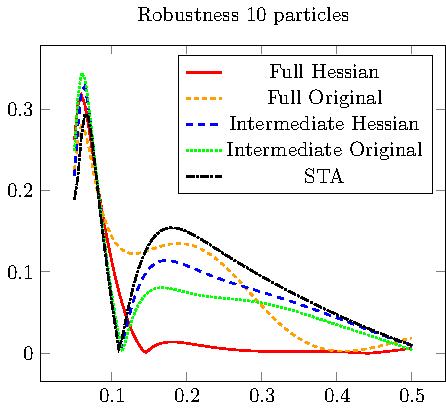
\includegraphics{./gfx/robustness_np10_nlambda5.pdf}
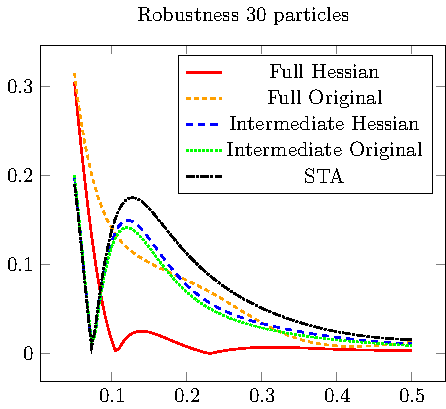
\includegraphics{./gfx/robustness_np30_nlambda5.pdf}

\begin{center}
    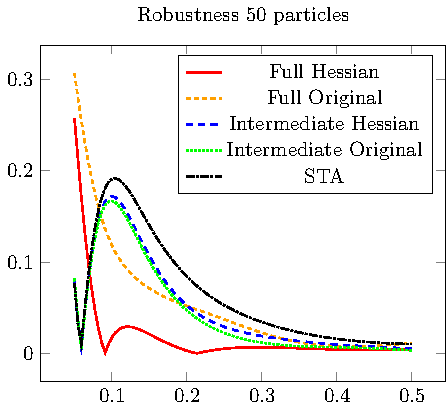
\includegraphics{./gfx/robustness_np50_nlambda5.pdf}
\end{center}

Again we can see that the best performances are achieved by the Hessian version of the eSTA protocol when applied to the full Hamiltonian of the system.

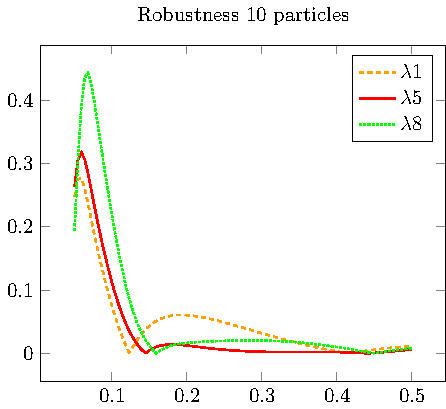
\includegraphics{./gfx/robustness_compare10.pdf}
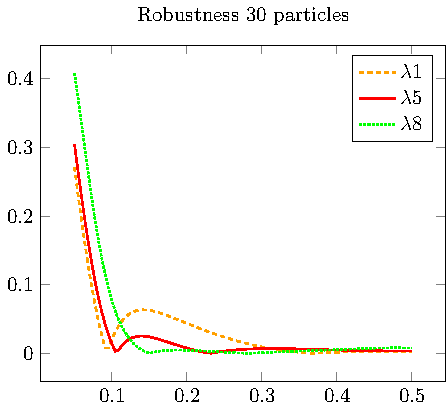
\includegraphics{./gfx/robustness_compare30.pdf}
\begin{center}
    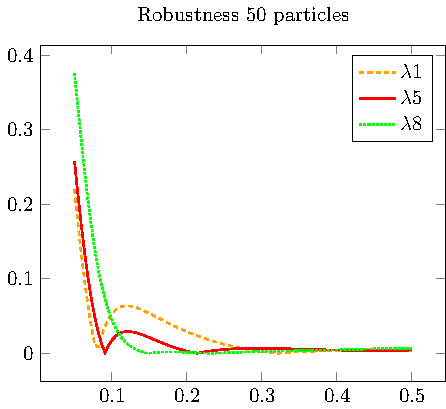
\includegraphics{./gfx/robustness_compare50.pdf}
\end{center}
